\documentclass[]{article}
\usepackage[utf8]{inputenc}
\usepackage[slovak]{babel}
\usepackage[hidelinks]{hyperref}
\usepackage{graphicx}
\usepackage{amsmath}
\newcommand*\textfrac[2]{
	\frac{\text{#1}}{\text{#2}}
}

\begin{document}
	
	\begin{titlepage}
		\begin{center}
			\textsc{{\LARGE Vysoké učení technické v~Brně\\[0.3em]
					Fakulta informačních technologií}}\\
			\vspace{\stretch{0.382}}
			{\Huge \textbf{Vplyv rozlíšenia a jasu na detekciu tváre}\\[0.5em]}
			\Large{Biometrické systémy}
			\vspace{\stretch{0.618}}
		\end{center}
		
		{\noindent \large Lukáš Dekrét\\Dávid Bolvanský}
	\end{titlepage}
	
	\section{Úvod}
	Cieľom tohto projektu bolo preskúmať vplyv rozlíšenia a jasu na úspešnosť detekcie tvárí. Bolo vybraných 5 nástrojov na detekciu tvárí, ktoré sú momentálne najpoužívanejšie a najpopulárnejšie. Na vybranom datasete fotografií sme vykonali niekoľko experimentov, kde sme skúšali meniť rozlíšenie/jas fotografií a sledovali sme, aký vplyv má táto zmena na detektory a ich úspešnosť v~detekcií tvárí.
	
	\section{Dataset a výber fotografií na experimenty}
	Na účely experimentovania sme si vybrali dataset \textit{Face Detection Data Set and Benchmark  (FBBD)} \footnote{\url{http://vis-www.cs.umass.edu/fddb/}}, ktorý bol navrhnutý na skúmanie problému detekcie tvárí.
	Z~tohto datasetu sme vybrali 100 fotografií, na ktorých sa nachádzala len jedna tvár, a táto tvár mala fixnú pixelovú šírku tváre \-- 90 pixelov. Výber fotografií mal takéto obmedzenia hlavne z~dôvodu experimentovania a stanovania si základných parametrov, ktoré fotografie budú mať. Použitie fixnej pixelovej dĺžky tvárí bolo odporúčané najmä pre experimenty zo zmenami rozlíšenia.
	V~našom výbere fotografií na experimentovanie sme snažili mať čo najviac vyvážené rasové rozloženie, no kvôli prechádzajúcimi obmedzeniam a nedostatku takýchto fotografií toto rovnomerné rozloženie nebolo možné úplne dosiahnuť. Výsledných 100 fotografií tak obsahuje 72 osôb europoidnej rasy, 14 osôb mongoloidnej rasy a 14 osôb negroidnej rasy. Pre účely zisťovania \textit{true negative} prípadov sme si našli 14 ďalších fotografií, kde nie sú ľudské tváre, no obsahujú objekty, ktoré pripomínajú ľudskú tvár (\textit{falošné tváre}). Dataset \textit{FBBD} obsahuje aj anotácie pre niektoré fotografie, no pre väčšinu našich vybraných fotografií informáciu o~\textit{ROI} žiaľ neposkytoval.
	
	\section{Výber nástrojov na detekciu tvárí}
	
	Vybrali sme nasledovných 5 nástrojov, s~ktorými sme následne prevádzali experimenty, a zisťovali ako obstoja v~netradičných / menej ideálnych podmienkach.
	
	\subsection*{MTCNN}
	Momentálnu \textit{state-of-the-art} detekciu tvári je možné dosiahnuť pomocou \textit{Multi-task Cascade Convolutional Neural Network}. Táto metóda bola predstavená v~článku \textit{Joint Face Detection and Alignment using Multi-task Cascaded Convolutional Networks} \footnote{\url{https://arxiv.org/pdf/1604.02878.pdf}}. Pri spracovaní daného obrázku ho spočiatku zmeníme v~rôznych mierkach, aby sme vytvorili obrazovú pyramídu, ktorá je vstupom nasledujúcej trojstupňovej kaskádovej štruktúry. 
	
	\newpage
	\noindent Existujú tri stupne klasifikácie:
	
	\begin{itemize}
		\item \textbf{1. fáza}
		
		Využíva sa plne konvolučná sieť, nazývaná návrhová sieť (P-Net), aby sme získali kandidátne tváre a ich regresné vektory ohraničujúceho obdlĺžnika. Potom sú kandidáti kalibrovaní na základe odhadovaných ohraničujúcich regresných vektorov. Následne použijeme nemaximálne potlačenie (non maximum suppression NMS) na zlúčenie vysoko prekrývajúcich sa kandidátov.
		
		\item \textbf{2. fáza}
		Všetci kandidáti sú presmerovaní do inej siete CNN, ktorá sa nazýva rafinovaná sieť (R-Net), ktorá ďalej odmieta veľké množstvo falošných kandidátov, vykonáva kalibráciu s~regresiou ohraničovacieho obdĺžnika a vykonáva NMS.
		
		\item \textbf{3. fáza}
		
		Táto fáza je podobná druhej fáze, až na to, že sa zameriavame na identifikáciu tvárových regiónov s~väčším dohľadom. Výstup siete je päť pozícií orientačných bodov tváre.
	\end{itemize}

	\subsection*{Haar}
	
	Detekcia objektov pomocou Haar kaskádového klasifikátora založeného na znakoch, je efektívna metóda vytvorená Paulom Violom a Michaelom Jonesom predstavená v~článku \textit{Rapid Object Detection using a Boosted Cascade of Simple Features} \footnote{\url{https://www.cs.cmu.edu/~efros/courses/LBMV07/Papers/viola-cvpr-01.pdf}}. Používa prístup strojového učenia, kde kaskádovitá funkcia je trénovaná z~veľa pozitívnych a negatívnych obrázkov. Následne je použítá na detekciu objektov v~iných obrázkoch. Algoritmus spočiatku potrebuje veľa pozitívnych obrazov (obrázky tvárí) a negatívnych obrazov (obrázky bez tvárí), aby mohol trénovať klasifikátor. Potom z~toho musí extrahovať znaky, kde každý znak je jedna hodnota získaná odpočítaním súčtu pixelov pod bielym obdĺžnikom (vybraná plocha na tváry) od súčtu pixelov pod čiernym obdĺžnikom (plocha na tváry pri bielom obdĺžniku). OpenCV poskytuje tréningovú metódu a vopred natrénované modely. Predpracované modely sú umiestnené v~dátovom priečinku pri inštalácii OpenCV.
	
	\subsection*{HoG}
	
	Histogram orientovaných gradientov (HOG) je deskriptor funkcie používaný v~počítačovom videní a spracovaní obrazov na účely detekcie objektov. Táto technika počíta výskyt gradientovej orientácie v~lokalizovaných častiach obrázka. Táto metóda je podobná metóde histogramov orientácie hrán, deskriptorov transformácie prvkov bez zmeny mierky a kontextov tvarov, líši sa však tým, že sa počíta na hustej mriežke rovnomerne rozmiestnených buniek a na zlepšenie presnosti sa používa prekrývajúca sa normalizácia lokálneho kontrastu. Základnou myšlienkou deskriptora histogramu orientovaných gradientov je to, že vzhľad a tvar lokálneho objektu v~obraze možno opísať rozložením gradientov intenzity alebo smerov okrajov. Obrázok je rozdelený na malé spojené oblasti nazývané bunky a pre pixely v~každej bunke je zostavený histogram smerov gradientu. Deskriptor je zreťazenie týchto histogramov. Pre lepšiu presnosť môžu byť lokálne histogramy normalizované kontrastom vypočítaním miery intenzity vo väčšej oblasti obrazu, nazývanej blok, a potom pomocou tejto hodnoty normalizovať všetky bunky v~bloku. Táto normalizácia vedie k~menšej zmene v~osvetlení a zatienení.
	
	\subsection*{CNN}
	
	Pri hlbokom učení je konvolučná neurónová sieť (\textit{Convolutional Neural Network}) triedou hlbokých neurónových sietí, ktoré sa najčastejšie používajú na analýzu vizuálnych snímok. CNN je regularizovaná verzia viacvrstvových perceptrónov. Viacvrstvové perceptróny obvykle znamenajú plne prepojené siete, čo znamená, že každý neurón v~jednej vrstve je pripojený ku všetkým neurónom v~ďalšej vrstve. „Plná prepojenosť“ týchto sietí ich robí náchylnými k~nadmernému spracovávaniu údajov. Medzi typické spôsoby regularizácie patrí pridanie určitej formy merania hmotnosti do stratovej funkcie. CNN však majú odlišný prístup k~regularizácii: využívajú hierarchický vzorec v~údajoch a zostavujú zložitejšie vzorce s~použitím menších a jednoduchších vzorov. Konvolučné siete boli inšpirované biologickými procesmi v~tom, že vzor konektivity medzi neurónmi pripomína organizáciu zvieracej vizuálnej kôry. CNN používa relatívne malé predspracovanie v~porovnaní s~inými algoritmami klasifikácie obrázkov.
	
	\subsection*{DNN}
	
	Hlboká neurónová sieť (\textit{Deep Neural Netvork}) je umelá neurónová sieť (\textit{Artificial Neural Network, ANN}) s~viacerými vrstvami medzi vstupnou a výstupnou vrstvou. DNN nájde správnu matematickú formulu, aby premenil vstup na výstup, či už ide o~lineárny alebo nelineárny vzťah. Sieť sa pohybuje po vrstvách a počíta pravdepodobnosť každého výstupu. Napríklad DNN, ktorá je trénovaná na rozpoznávanie ľudských tvárí, prejde daný obrázok a vypočíta pravdepodobnosť, že ľudské tváre sú na obrázku. Užívateľ môže skontrolovať výsledky a zvoliť, ktoré pravdepodobnosti by sieť mala zobraziť (za použitia prahov atď.) A~vrátiť navrhované priradenie. Každá matematická formula ako taká sa považuje za vrstvu. Komplexná DNN má veľa vrstiev, preto názov „hlboké“ siete.
	DNN môžu modelovať komplexné nelineárne vzťahy. Architektúry DNN generujú kompozičné modely, kde je objekt vyjadrený ako vrstvená kompozícia primitívov. Dodatočné vrstvy umožňujú zloženie spodných vrstiev a potenciálne modelujú komplexné údaje s~menším počtom jednotiek ako podobne vykonávaná plytká sieť.
	
	\newpage
	Použili sme nasledovné implementácie detektorov: 
	
	\begin{itemize}
		\item \textbf{MTCCN}
		
		\url{https://github.com/ipazc/mtcnn}
		
		\item \textbf{Haar}
		
		\url{https://docs.opencv.org/3.4/db/d28/tutorial_cascade_classifier.html}
		
		\item \textbf{HoG}
		
		\url{https:/dlib.net/}
		
		\item \textbf{CNN}
		
		\url{https:/dlib.net/}
		
		\item \textbf{HoG}
		
		\url{https://www.cvlib.net/}
	\end{itemize}
	
	\section{Experimenty}
	
	Vybraných 100 fotiek sme rozčlenili do priečinkov podla rasovej príslušnosti osôb na fotografiách. Pre každú rasu sme zisťovali vplyv zmeny rozlíšenia a jasu na úspešnosť detekcie tvárí. Zobrali sme aj 14 fotografií, ktoré neobsahovali ľudské tváre, ale obsahovali niečo, čo sa na ľudské tváre môže podobať, a skúmali sme, či nástroje správe odhalia tento fakt. Nakoniec sme zobrali všetkých 100 fotiek, pridali sme k~nim týchto 14 fotografií, a urobili celé meranie aj pre túto sadu fotografií.
	
	Pomocou vytvoreného skriptu sme vytvorili nové obrázky, ktoré mali znížené rozlíšenie. Detektory sa pokúšali hladať tváre na fotografiách, ktoré boli 10, 20, 30, 40, 50, 60, 80 a 100 \% pôvodných fotografií. Vytvorili sme aj nové zosvetlené / stmavené fotografie, ktoré mali rôznu úroveň jasu. Vyskúšali sme 4 úrovne zosvetlenia (faktor jasu $>$ 1) a 4 úrovne stmavenia (faktor jasu $<$ 1) fotografií. Následne sme pristúpili k~meraniu úspešnosti detekcie tvárí pomocou vyššie uvedených nástrojov. Na meranie výkonnosti detektorov sme použili metriku \textit{Accuracy}.
	
	Presnosť (\textit{Accuracy}) je jedna z~metrík pre hodnotenie klasifikačných modelov. Formálne má presnosť nasledovnú definíciu:
	\begin{center}
		Presnosť = $\textfrac{počet správnych predikcií}{celkový počet predikcií}$
	\end{center}
	Pre binárnu klasifikáciu sa presnosť môže vypočítať aj z~hľadiska pozitívnych a negatívnych prípadov takto:
	\begin{center}
		Presnosť = $\textfrac{true positive + true negative}{true positive + true negative + false positive + false negative}$
	\end{center}
	Ak detektor nenašiel tvár na fotografií, zaznamenali sme si to ako \textit{false negative}, v~prípade falošných tvarí ako \textit{true negative} prípad. V~prípade, že detektor našiel jednu alebo viac tvárí na fotografií, kde nebola ľudská tvár, všetky výskyty sa rátali ako \textit{false positive} prípady. Ak našiel jednu alebo viac tvárí na fotografii so skutočnou ľudskou tvárou, jeden prípad sa započítal ako nájdenie tváre (\textit{true positive} prípad) a ostatné výskyty ako \textit{false positive} prípady. Ako sme vyššie uviedli, pre naše fotografie neboli dostupné \textit{ROI} informácie \-- ak by boli, bolo by možné použiť metriku \textit{Intersection over union (IoU)} spolu s~nejakou hranicou dobrej predikcie a lepšie stanoviť, či jedna z~nájdených tvári je naozaj tá správna.
	
	
	\subsection*{Vplyv rozlíšenia na presnosť detekcie tvárí}
	
	Okrem našich experimentov v~tejto správe sú dostupné aj iné relavantné vedecké články, ktoré sa tiež venujú vplyvu rozlíšenia na detekciu tvárí, a to napríklad \textit{Effects of Image Resolution on Automatic Face Detection} \footnote{\url{https://ieeexplore.ieee.org/document/8680985}}, \textit{The Effect of Image Resolution on the Performance of a Face Recognition System} \footnote{\url{https://ieeexplore.ieee.org/document/4150409}} a \textit{Face Recognition Vs Image Resolution} \footnote{\url{https://ieeexplore.ieee.org/document/1598563}}
	
	\subsubsection*{Europoidná rasa}
	
	\begin{figure}[h!]
		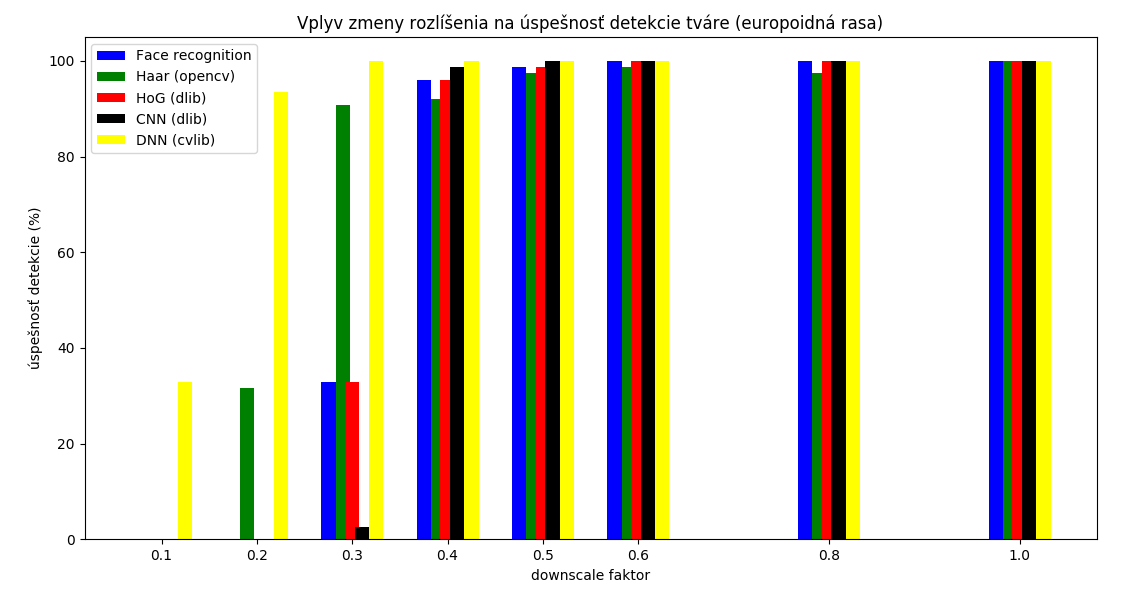
\includegraphics[height=6cm, width=\textwidth]{Vysledky_rozslisenie/europ/Figure_1.png}
		\caption{Vplyv rozlíšenia na presnosť detekcie tvárí osôb europoidnej rasy}
	\end{figure}

	
	\newpage
	\subsubsection*{Mongoloidná rasa}
	\begin{figure}[h!]
		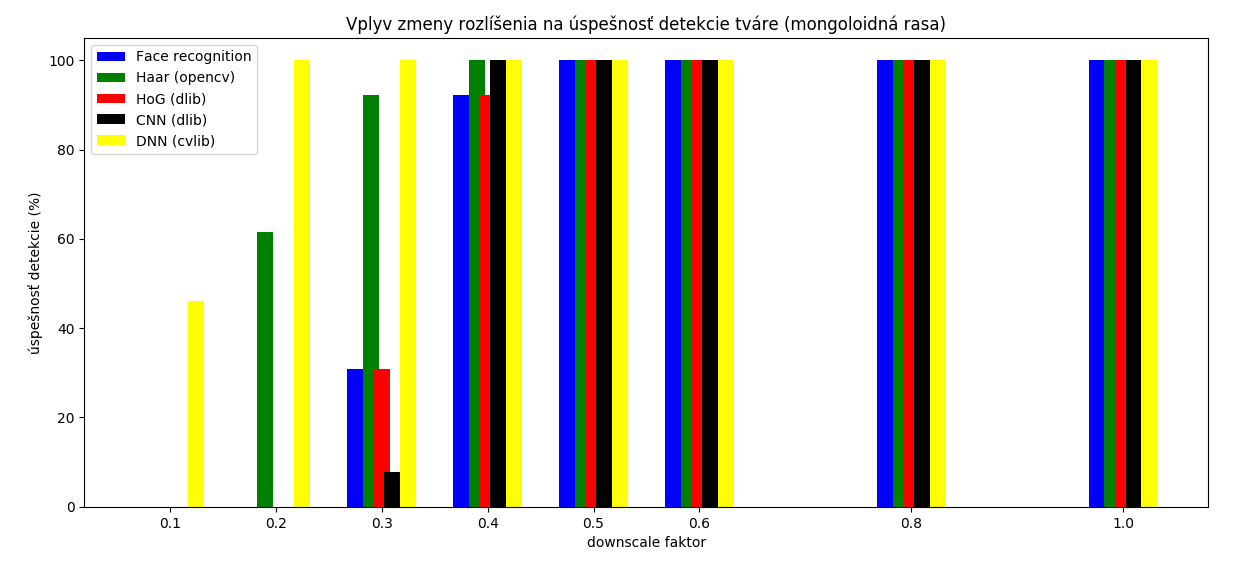
\includegraphics[height=6cm,width=\textwidth]{Vysledky_rozslisenie/mongo/Figure_1.png}
		\caption{Vplyv rozlíšenia na presnosť detekcie tvárí osôb mongoloidnej rasy}
	\end{figure}

	Z~grafov vidíme, že výsledky presnosti detektorov sú veľmi podobné medzi mongoloidnou a europoidnou rasou. Všetky detektory si vedú veľmi dobre aj pri fotografiách, ktoré sú len 40 \% ich pôvodnej veľkosti. Za touto hranicou potvrdzujú DNN a MTCNN, že sa jedná o~momentálne \textit{state-of-the-art} detektory tvárí a aj pri veľmi malých fotografiách dokážu nájsť tváre.

	\subsubsection*{Negroidná rasa}
	\begin{figure}[h!]
		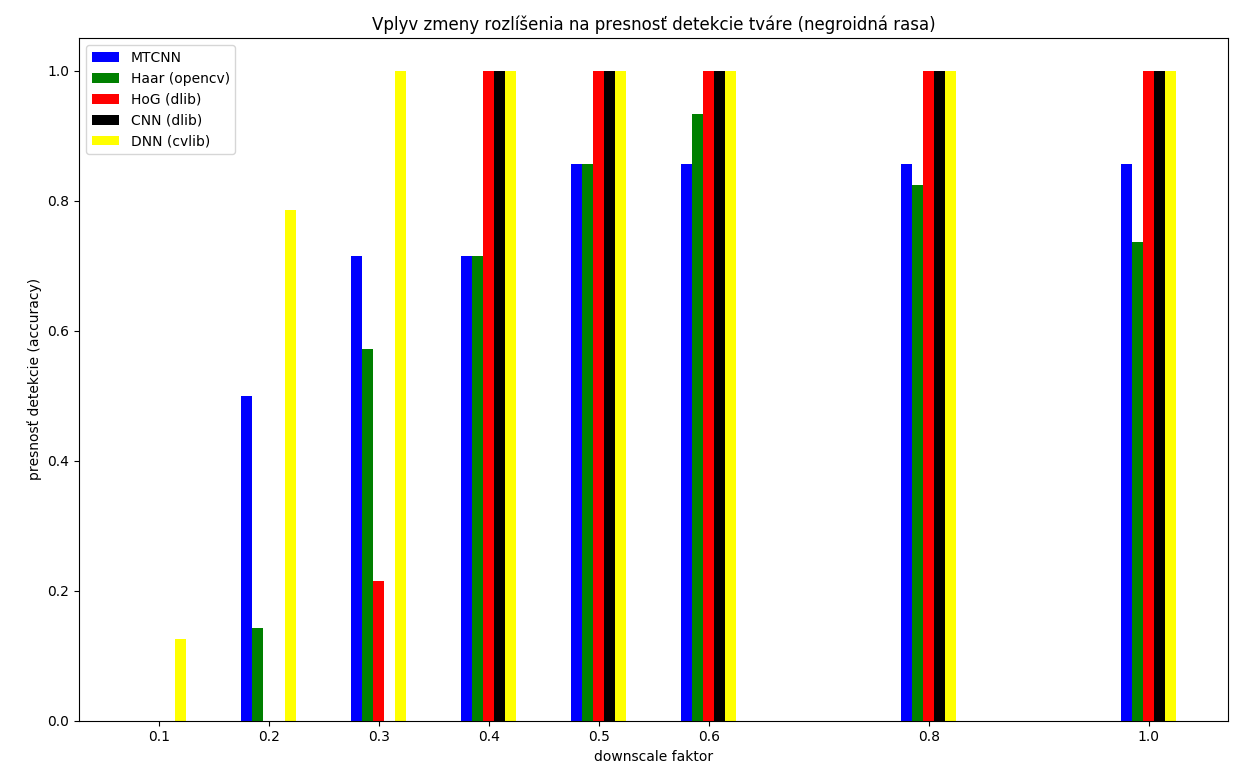
\includegraphics[height=6cm,width=\textwidth]{Vysledky_rozslisenie/negro/Figure_1.png}
		\caption{Vplyv rozlíšenia na presnosť detekcie tvárí osôb negroidnej rasy}
	\end{figure}

	\newpage
	U~negroidnej rasy je však možné zaznamenať, že presnosť detektora MTCNN sa u~tejto rasy znížila. Trénovacia sada zrejme obsahovala málo osôb tejto rasy.
	
	\subsubsection*{Falošné tváre}
	\begin{figure}[h!]
		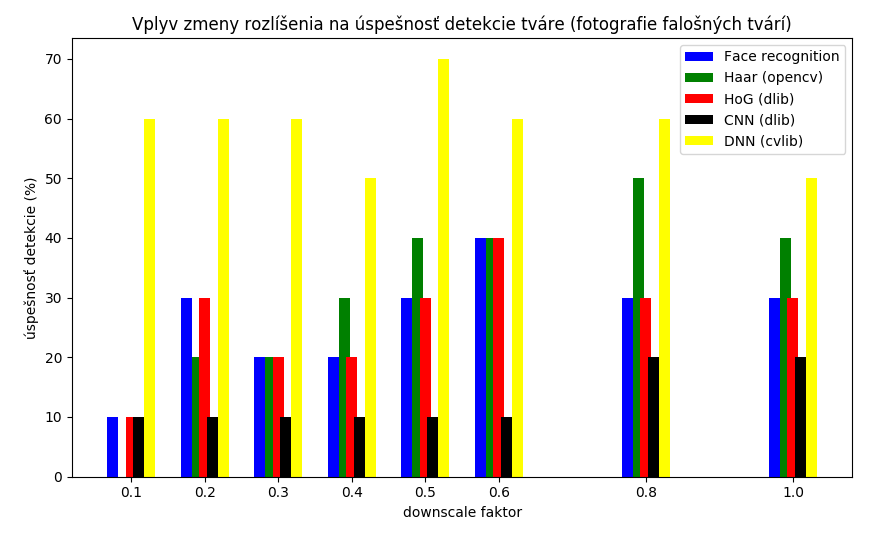
\includegraphics[height=6cm,width=\textwidth]{Vysledky_rozslisenie/fake/Figure_1.png}
		\caption{Vplyv zmeny rozlíšenia na presnosť detekcie tvárí - falošné tváre}
	\end{figure}

	Vidíme, že detektory MTCNN, HoG, CNN je možné ľahko oklamať fotografiami falošných tvárí, a s~menšími rozlíšeniami sa situácia len zhoršuje. Haar je mierne od nich lepší, no detektor DNN je u~tohto experimentu jasný vítaz.
	
	\subsubsection*{Všetky rasy a falošné tváre}
	\begin{figure}[h!]
		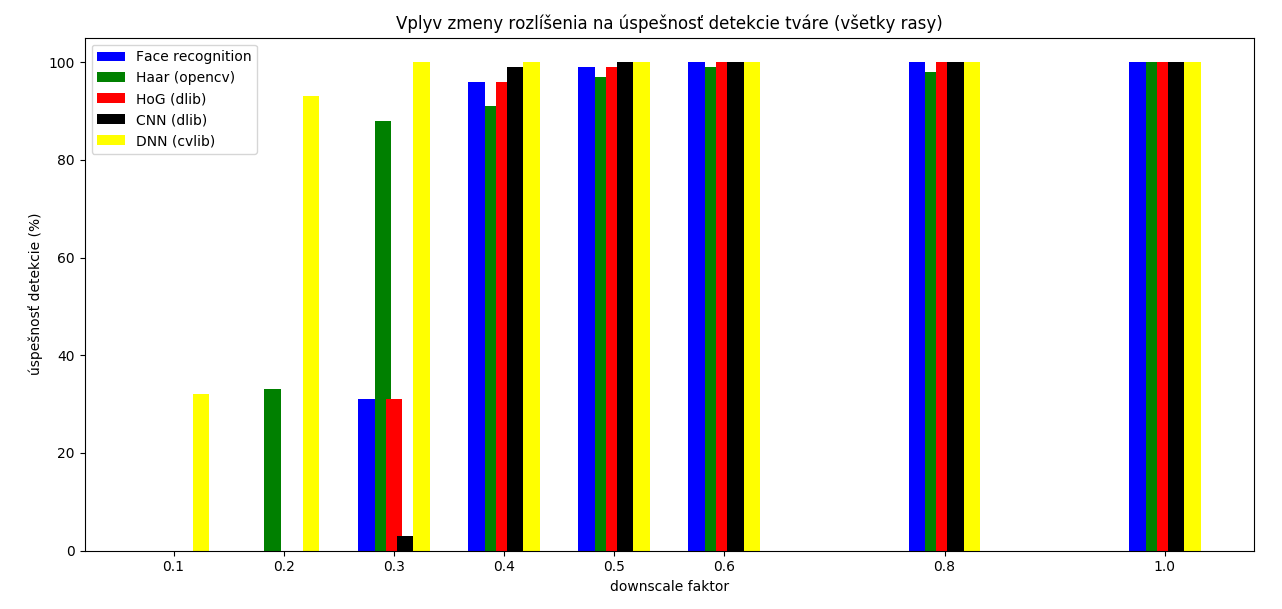
\includegraphics[height=5.6cm,width=\textwidth]{Vysledky_rozslisenie/all/Figure_1.png}
		\caption{Vplyv rozlíšenia na presnosť detekcie tvárí \-- všetky rasy a falošné tváre}
	\end{figure}

	Celkovo môžeme zhodnotiť, že všetky detektory sú dosť presné aj pri malých rozlíšeniach. Pri veľmi malých rozlíšeniach sú ale v~súčasnej dobe najlepšie MTCNN a DNN.
	Situácia u~ostatných detektorov by mohla byť lepšia, ak by boli natrénované na inom datasete alebo spustené s~inými parametrami. Graf ukazuje aj niektoré zaujímave a možno na prvý pohľad prekvapivé výsledky, najmä v~prípade detektorov CNN, HoG a Haar. 
	
	Predtrénovaná CNN umožňuje dobre detegovať tváre len ak je rozlíšenie tváre na fotografiách s~rozlíšením aspoň 80x80 pixelov. Implementácia CNN v~dlib umožňuje nastaviť parameter \texttt{upsample count}, ktorý môže pomôcť pri malých fotografiách \-- odporúčaná hodnota je 1. Na grafoch si je možné všimnúť zaujímavý pád presnosti CNN na rozmedzí 30 a 40 \%, čo však je možné vysvetliť nasledovne: 40 \% z~našej fixnej šírky tváre (90px) je 36px, po 1x upsample dosahujeme už spomínané minimálne rozlíšenie 80x80. V~prípade 30 \% je teda jasné, že sa už nachádzame pod touto hranicou a detekcia tvári je veľmi slabá (čo namerané výsledky plne potvrdzujú). Presnosť detekcie u~CNN je možné zlepšiť zmenou parametru \texttt{upsample count} na vyššie číslo, no doba potrebná na detekciu tváre za znateľne zvýši, čo môže byť už problematické na reálne použitie. Toto vysvetlenie platí aj pre HoG, keďže aj tu bola použitá hodnota 1 ako \texttt{upsample count} a aj u~HoG z~dlib platí, že umožňuje dobre detegovať tváre len ak je rozlíšenie tváre na fotografii aspoň 80x80.

	Ako už bolo spomenuté, Haar je založený na princípe obrázkovej pyramídy, ktorá je tvorená na základe \textit{scale faktoru}. Pre experimenty sme použili model \texttt{haarcascade\_frontalface\_default.xml}, ktorý je trénovaný na obrázkoch v~rozlíšení 24x24. Hodnota \textit{scale faktoru} 1.1 (ktorá je predvolená v~implementácii Haar v~OpenCV) určuje, že obrázok je medzi dvoma vrstvami redukovaný o~10 \% (tj. faktor definuje koľko vrstiev bude). Zmenou \textit{scale faktor} parametru je teda možné zlepšiť presnosť detekcie, no podobne ako u~CNN, zmena tohto parametra za účelom zvýšenia presnosti prináša so sebou aj zvýšenie doby potrebnej na detekciu tváre. 
	
	\subsection*{Vplyv jasu na presnosť detekcie tvárí}
	
	Okrem našich experimentov v~tejto správe sú dostupné aj iné relavantné vedecké články, ktoré sa tiež venujú vplyvu jasu na detekciu tvárí, a to napríklad \textit{Face detection and the effect of contrast and brightness} \footnote{\url{https://www.researchgate.net/publication/290861830_Face_detection_and_the_effect_of_contrast_and_brightness}} a 
	\textit{Factor Analysis in Unconstrained Viola-Jones Face Detection: Brightness, Contrast, Focus Measure, Eyewear, Gender, and Occlusion} \footnote{\url{https://www.osti.gov/servlets/purl/1468194}}
		
	\subsubsection*{Europoidná rasa}
	
	\begin{figure}[h!]
		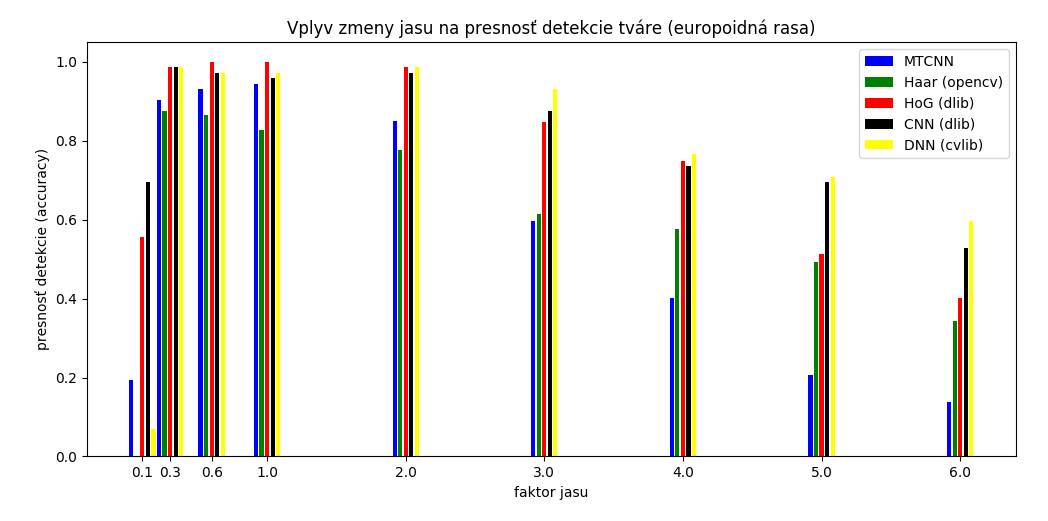
\includegraphics[width=\textwidth]{Vysledky_jas/europ/Figure_1.png}
		\caption{Vplyv jasu na presnosť detekcie tvárí osôb europoidnej rasy}
	\end{figure}

	Detektori CNN a DNN bol u~osôb europoidnej rasy výrazne lepšie od ostatných detektorov pri vysokých úrovniach zosvetlenia fotografie.

	\subsubsection*{Mongoloidná rasa}
	\begin{figure}[h!]
		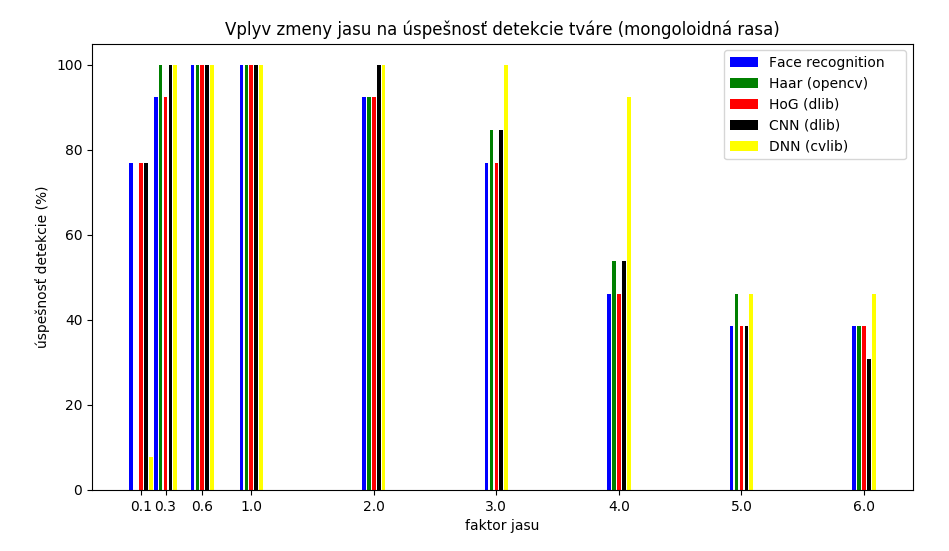
\includegraphics[width=\textwidth]{Vysledky_jas/mongo/Figure_1.png}
		\caption{Vplyv jasu na presnosť detekcie tvárí osôb mongoloidnej rasy}
	\end{figure}

	Detektor DNN bol u~osôb mongoloidnej rasy výrazne lepší od ostatných detektorov pri vysokej úrovni zosvetlenia fotografie. Vidíme, že vysoké zosvetlenie nemalo až tak výrazný vplyv na presnosť detekcie u~tejto rasy v~porovnaní s~ostatnými rasami \-- jednoducho povedané, osoby s~tmavou pokožkou sa javili ako belosi pred detekormi.

	\newpage

	\subsubsection*{Negroidná rasa}
	\begin{figure}[h!]
		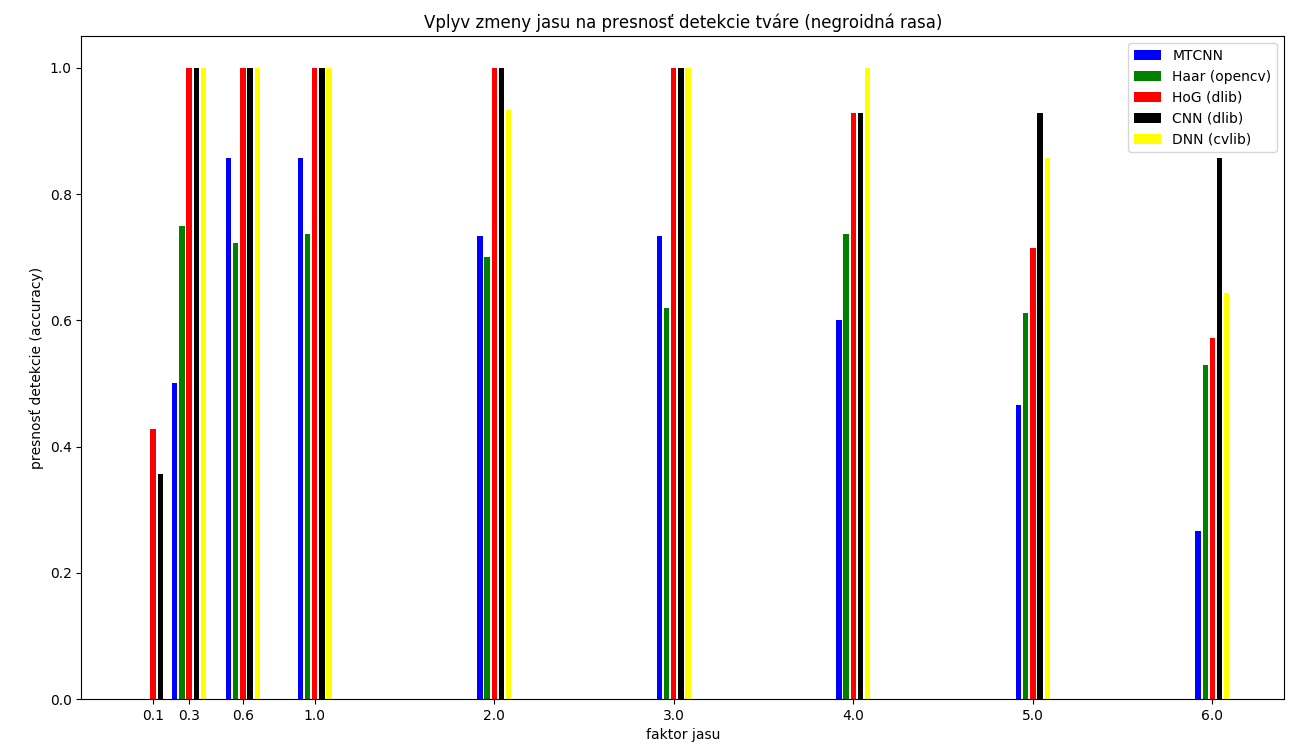
\includegraphics[width=\textwidth]{Vysledky_jas/negro/Figure_1.png}
		\caption{Vplyv jasu na presnosť detekcie tvárí osôb negroidnej rasy}
	\end{figure}

	Detektor CNN bol u~osôb negroidnej rasy mierne lepší ako DNN.

	\subsubsection*{Falošné tváre}
	\begin{figure}[h!]
		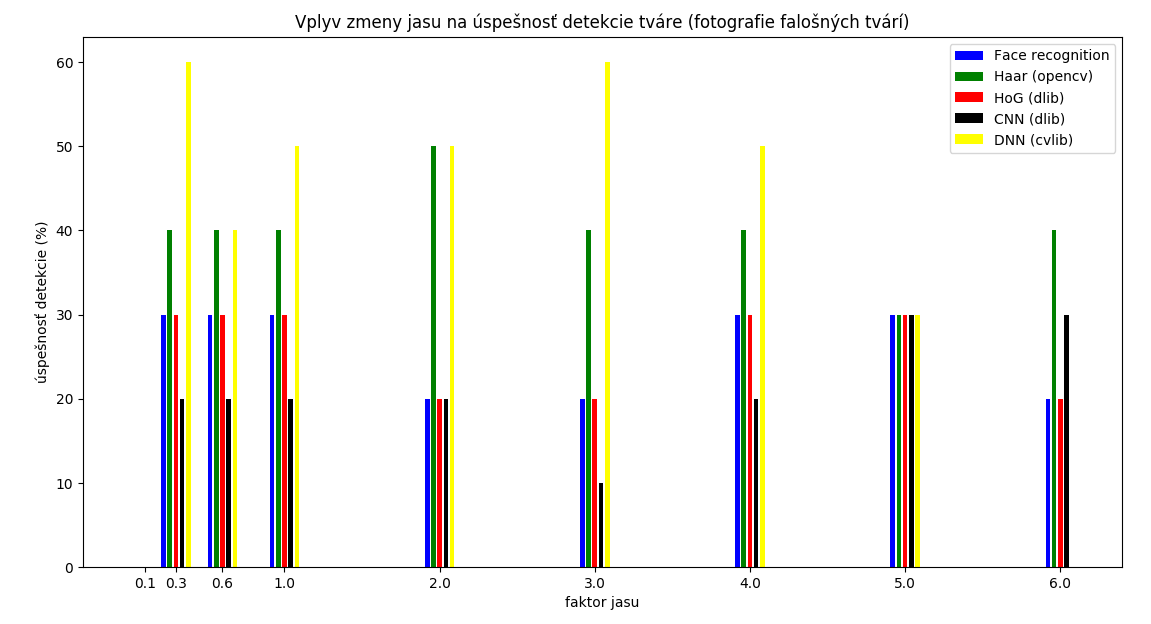
\includegraphics[width=\textwidth]{Vysledky_jas/fake/Figure_1.png}
		\caption{Vplyv jasu na presnosť detekcie tvárí \-- falošné tváre}
	\end{figure}

	Detektor DNN potvrdil, to čo ukazoval trend z~podobného merania u~zmeny rozlíšenia, a nedal sa oklamať falošnými tvárami. V~tom prípade avšak Haar dokázal poraziť DNN. Skôr je ale pravdepodobné, že Haar jednoducho nič na tých fotografiách detegovať nevedel. Detektory MTCNN, HoG, CNN sa dali veľmi ľahko oklamať falošnými tvárami.
	
	\subsubsection*{Všetky rasy a falošné tváre}
	\begin{figure}[h!]
		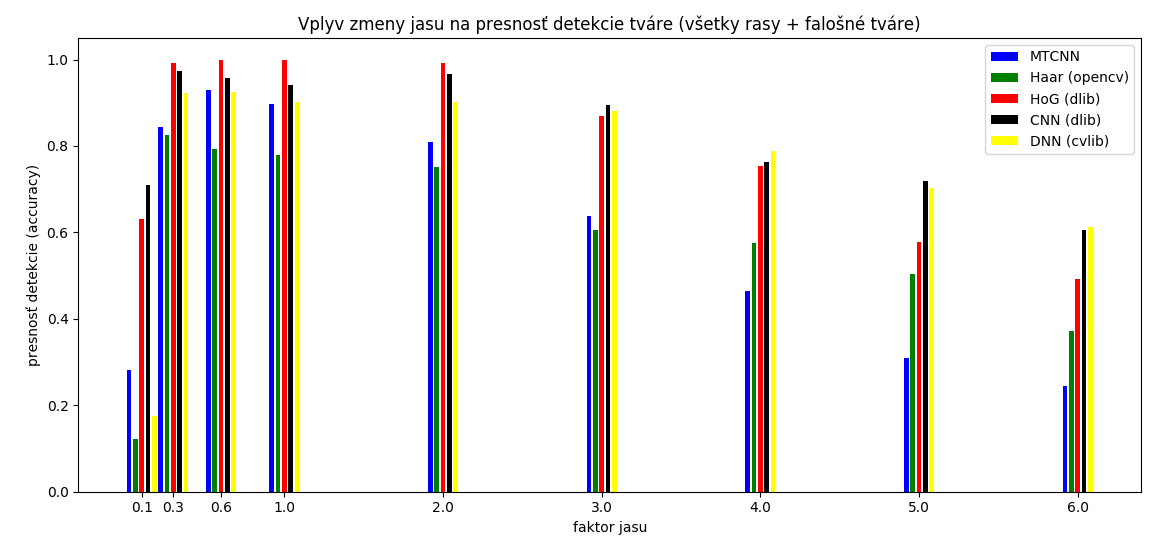
\includegraphics[width=\textwidth]{Vysledky_jas/all/Figure_1.png}
		\caption{Vplyv jasu na presnosť detekcie tvárí - všetky rasy a falošné tváre}
	\end{figure}

	Celkovo môžeme zhodnotiť, že detektory v~prípade zmeny jasu začali byť značne neúspešné až pri veľmi nízkej úrovni zosvetlenia / stmavenia. U~týchto meraní sa výraznejšie vyčlenila skupina detektorov HoG, CNN, DNN, ktorá bola výrazne presnejšia v~detekcii tvárí ako Haar a MTCNN. Zmena jasu predstavuje pre Haar značný problém. Môže za to práve spôsob extrakcie znakov, ktorý vzniká rozdielom súčtu pixelov na daných plochách. Keďže menia hodnoty pixelov, zmenia sa aj súčty pixelov zmenia, a teda aj ich rozdiel, čo má za následok iný výsledný vektor znakov. Je celkom prekvapivé, že MTCNN ako momentálne jeden z~\textit{state-of-the-art} detektorov tvárí dopadol najhoršie. Vidíme, že najmä vyššie úrovne zosvetlenia boli pre tento detektor veľkým problémom.
	
	\section{Záver}
	
	Namerané dáta ukazujú, že zmena rozlíšenia nemá výraznejší vplyv na úspešnosť a presnosť detekcie, keďže detektory používajú techniky predspracovania fotografií (napr. \textit{rescaling}), ktoré pomáhajú eliminovať efekt vplyvu rozlíšenia na detekciu tvárí. Experimenty taktiež poukazujú na to, že niektoré detektory horšie zvládajú už aj mierne zmeny úrovne jasu, čo má negatívny vplyv na ich úspešnosť a presnosť v~detekcii tvárí. Dôležitým poznatkom je aj to, že presnosť detektorov dosť závisí od ich konfigurácie a zmena niektorých parametrov môže značne spresniť detekciu, aj keď za cenu, že samotná detekcia sa spomalí.
	
	
\end{document}